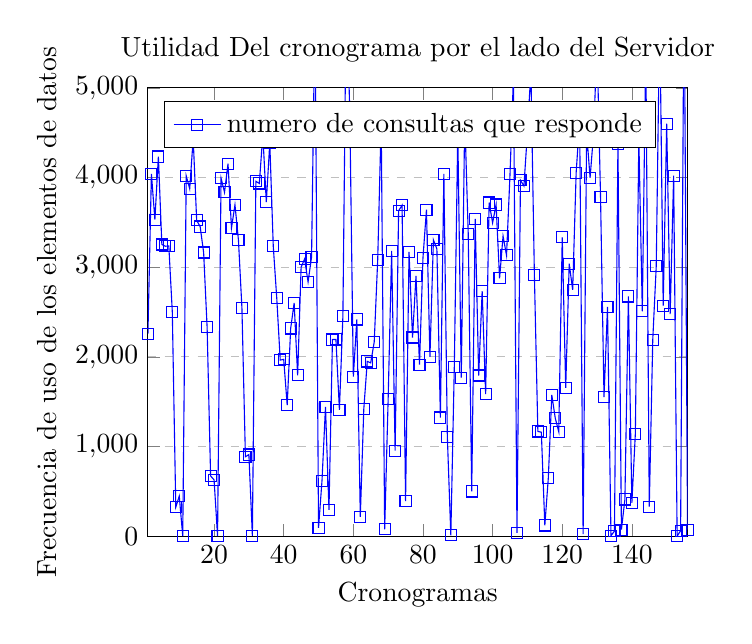
\begin{tikzpicture}
\begin{axis}[
    title={Utilidad Del cronograma por el lado del Servidor},
    xlabel={Cronogramas},
    ylabel={Frecuencia de uso de los elementos de datos},
    xmin=1, xmax=156,
    ymin=0, ymax=5000,
    xtick={},
    ytick={},
    legend pos=north west,
    ymajorgrids=true,
    grid style=dashed,
]

\addplot[
    color=blue,
    mark=square,
    ]
    coordinates {
%UTILIDAD TOTAL
%(cronograma, numero cues que usan al cronograma)
(1,2257)
(2,4041)
(3,3530)
(4,4234)
(5,3253)
(6,3234)
(7,3237)
(8,2503)
(9,323)
(10,447)
(11,2)
(12,4018)
(13,3875)
(14,4433)
(15,3522)
(16,3453)
(17,3164)
(18,2331)
(19,672)
(20,628)
(21,2)
(22,3994)
(23,3835)
(24,4155)
(25,3437)
(26,3696)
(27,3302)
(28,2545)
(29,886)
(30,910)
(31,4)
(32,3958)
(33,3934)
(34,4480)
(35,3725)
(36,4387)
(37,3234)
(38,2657)
(39,1964)
(40,1972)
(41,1461)
(42,2317)
(43,2601)
(44,1794)
(45,3000)
(46,3091)
(47,2836)
(48,3113)
(49,5953)
(50,93)
(51,620)
(52,1441)
(53,294)
(54,2193)
(55,2194)
(56,1410)
(57,2455)
(58,6203)
(59,4686)
(60,1779)
(61,2417)
(62,216)
(63,1416)
(64,1949)
(65,1933)
(66,2167)
(67,3084)
(68,4630)
(69,77)
(70,1531)
(71,3181)
(72,953)
(73,3629)
(74,3691)
(75,390)
(76,3170)
(77,2216)
(78,2902)
(79,1913)
(80,3105)
(81,3642)
(82,2000)
(83,3304)
(84,3204)
(85,1323)
(86,4042)
(87,1110)
(88,10)
(89,1887)
(90,4504)
(91,1768)
(92,4677)
(93,3374)
(94,499)
(95,3539)
(96,1792)
(97,2733)
(98,1585)
(99,3721)
(100,3495)
(101,3699)
(102,2875)
(103,3347)
(104,3132)
(105,4037)
(106,5139)
(107,36)
(108,3969)
(109,3906)
(110,4503)
(111,5189)
(112,2915)
(113,1168)
(114,1160)
(115,120)
(116,648)
(117,1575)
(118,1316)
(119,1165)
(120,3333)
(121,1655)
(122,3039)
(123,2747)
(124,4055)
(125,4642)
(126,23)
(127,4502)
(128,3998)
(129,4488)
(130,5503)
(131,3787)
(132,1552)
(133,2556)
(134,6)
(135,56)
(136,4374)
(137,73)
(138,410)
(139,2674)
(140,372)
(141,1142)
(142,4438)
(143,2508)
(144,5469)
(145,329)
(146,2190)
(147,3010)
(148,5848)
(149,2571)
(150,4601)
(151,2478)
(152,4021)
(153,0)
(154,61)
(155,6318)
(156,72)
(157,3228)
(158,6095)
(159,3814)
    };
    \legend{numero de consultas que responde}

\end{axis}
\end{tikzpicture}

